\section{Evaluation}
\label{sec:evaluation}

In this section, we present an evaluation of \name programming model
with the aim of assessing its practical utility for describing
geo-distributed eventually consistent applications. In particular, we
are interested in the horizontal scalability of applications built
using \name. Typical distributed eventually consistent data stores use
custom synchronization and dissemination protocols for transferring
updates between replicas. Unlike this, \name is realized over Irmin
which uses Git transfer protocol~\cite{..}, a protocol not designed
with distributed data stores in mind. Hence, we also evaluate the
performance of synchronization and merging.

\subsection{Benchmark: Collaborative editing}

In order to evaluate this, we have implemented a collaborative editing
application that simulates concurrent editing of the same document by several
authors. This application is not unlike Google Docs, but also differs from it
by the fact that we do not need a central server that coordinates the edits.
Instead, edits from each author is asynchronously sent to other authors. The
shared document itself is represented by a mergeable rope of characters
(Section~\ref{sec:model}), and hence, the remote edits can be correctly
reconciled into the local document. We resolve conflicts on concurrent
substitutions at the same position (such as two authors concurrently editing
\C{"abc"} to \C{"xbc"} and \C{"ybc"}, respectively) by choosing the character
with the smaller ASCII code. For the benchmarks, the initial document that we
use has 1576 characters. The workload consists of 4000 edit operations at
random indices with 85\% insertions and 15\% deletions.

\subsection{Experimental setup}

\begin{figure}[t]
  \centering
	\begin{subfigure}{0.45\textwidth}
		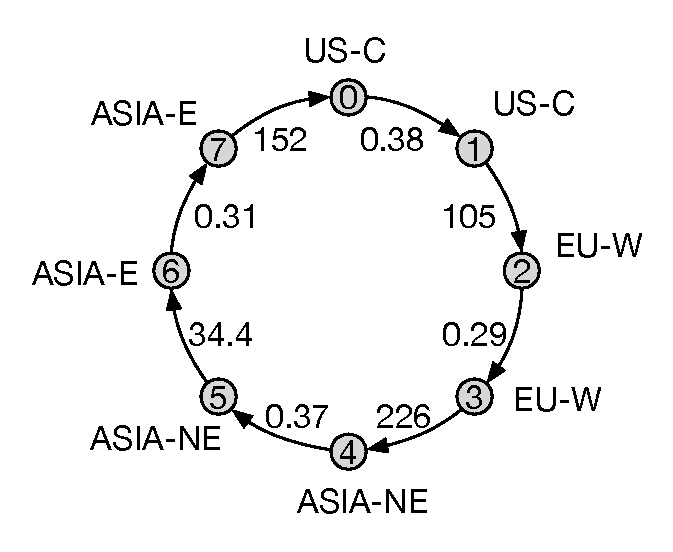
\includegraphics[width=0.9\textwidth]{Figures/cluster.pdf}
		\caption{8-node ring cluster on Google Cloud Platform used for
			benchmarking. US-C, EU-W, ASIA-NE and ASIA-E are availability zones
			us-central1-b, europe-west1-b, asia-northeast1-b and asia-east1-b
			respectively. Edge labels are inter-node latencies in milliseconds.}
		\label{fig:cluster}
	\end{subfigure}
	\hfill
	\begin{subfigure}{0.45\textwidth}
		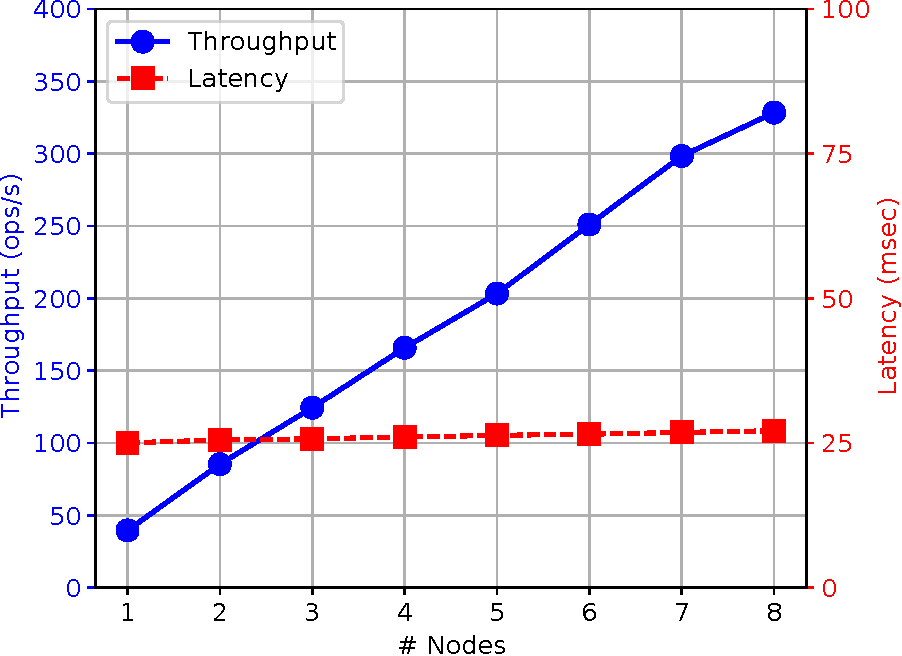
\includegraphics[width=\textwidth]{Graphs/scalability.pdf}
		\caption{Scalability: Overall throughput of the cluster and latency of each
			operation.}
		\label{grf:scalability}
	\end{subfigure}
	\par\bigskip
	\begin{subfigure}{0.45\textwidth}
		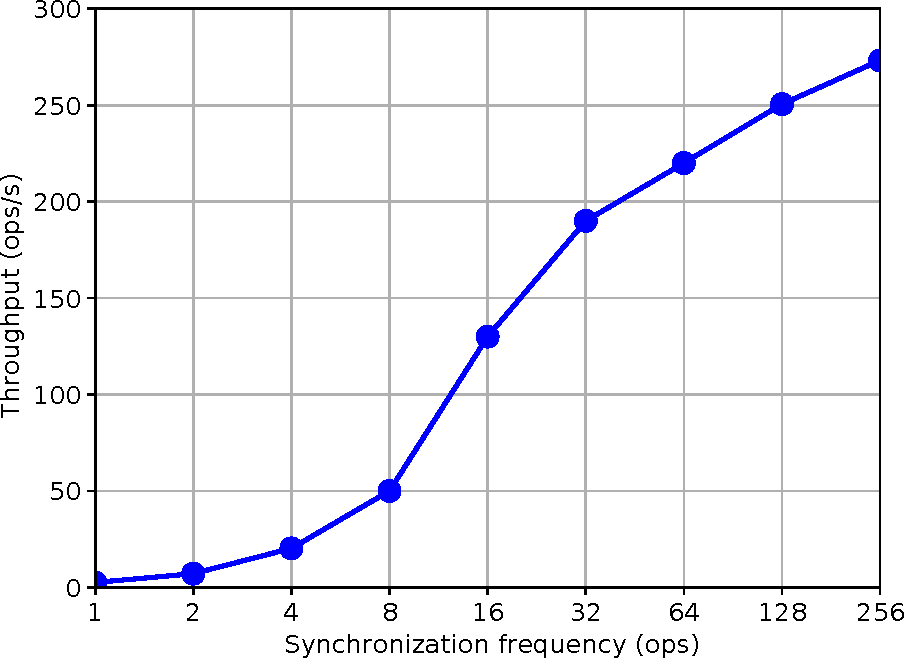
\includegraphics[width=\textwidth]{Graphs/synchronization.pdf}
		\caption{Synchronization: Overall throughput of the cluster while actively
			synchronizing with the successor node.}
		\label{grf:synchronization}
	\end{subfigure}
	\hfill
	\begin{subfigure}{0.45\textwidth}
		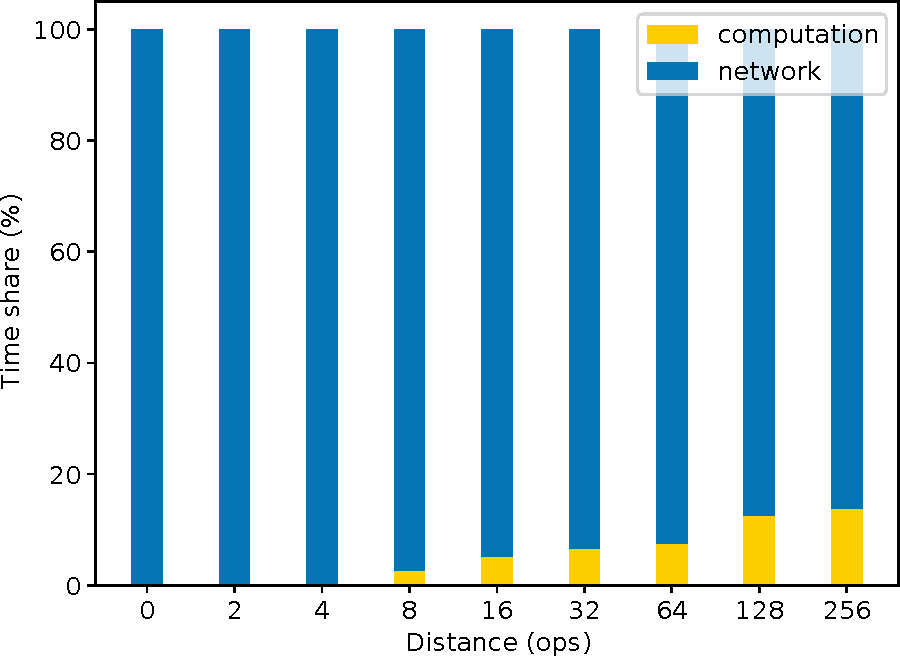
\includegraphics[width=\textwidth]{Graphs/merge.pdf}
		\caption{Merge performance: Cost of merging concurrent operations across
		nodes.}
		\label{grf:merge}
	\end{subfigure}
	\caption{\name performance evaluation.}
  \label{grf:evaluation}
\end{figure}

For our experiments, we instantiate an 8-node geo-distributed cluster in Google
Cloud Platform~\cite{gcp}. Each node is an \C{n1-standard-4} instance with 2
virtual CPUs and 7.5 GB of memory. The nodes are arranged in a ring as shown in
Figure~\ref{fig:cluster} and synchronize (push and pull updates) when necessary
with its successor. While \name does not impose any restrictions on
synchronizing with other nodes, we choose to only synchronize with the
successor since we are guaranteed eventual convergence with a ring cluster. If
the successor becomes unavailable, the node synchronizes with other available
nodes. Operations are generated and applied locally on each node before they
are propagated eventually to other nodes with the help of a background thread
that synchronizes with its successor every second.

\subsection{Results}

We evaluate the scalability of concurrent editing application by increasing the
cluster size from 1 to 8 (the 4 node ring cluster consists of nodes numbered 0
to 3), with each node performing concurrent edits to the same document. In each
case, we measure the overall cluster throughput and latency of each operation.
The results are presented in Figure~\ref{grf:scalability}. The results show
that the cluster throughput increases linearly with the number of concurrent
editors, while the latency for each operation remains the same. This is because
each operation is performed locally and does not require synchronization with
other nodes. The nodes remain available to accept requests even if the node
gets disconnected. Since the document type is mergeable, eventually when the
node comes back online, the updates are synchronized with the cluster.

While updates are propagated asynchronously, we also measured the impact of
propagating updates synchronously by forcing synchronization every few
operations. This corresponds to a partially synchronous system, which is also
unavailable; if the cluster is unreachable, local operations will not be
accepted. While this is not a realistic deployment, the results help us
understand the overhead of synchronization. The results are shown in
Figure~\ref{grf:synchronization}. The result show that frequent blocking
synchronization is prohibitively expensive with the throughput dropping to 3
ops/s for synchronizing after every operation. \name uses Git transfer protocol
for synchronization which involves multiple round trips between the nodes for
synchronization. But as the synchronizations get less frequent, we can see that
the throughput asymptotically approaches the asynchronous case
(Figure~\ref{grf:scalability}).

Finally, we evaluate the performance of merge functions. For this experiment,
we consider the nodes 1 (\C{us-central1-b}) and 2 (\C{europe-west1-b}). Both
nodes start with the initial document and perform \C{n} concurrent edits
without synchronization. After this, the nodes synchronize pushing the local
edits and pulling the remote edits, and merge to produce the final document. In
this case, we indicate the distance of synchronization as \C{2n}.
Figure~\ref{grf:merge} presents the time share between network and computation
for performing 3-way merge as we increase the operation distance between the
remote branches. We see that the merge time is dominated by the network
overhead. This is because of the transfer protocol involving multiple
round trips and the need to transfer objects not only for application objects
but also Git internal objects for history, directory structure and branches. We
observe that we can improve the network performance by implementing a streaming
protocol that eagerly transfers objects.

More importantly, the cost of computation grows sub-linearly. This is because
of efficient merge function on ropes~\ref{ropes} enabled by Irmin's
content-addressed storage backend, and more expensive operational
transformation of merging concurrent edits to leaf nodes~\ref{lists} is invoked
rarely on small. On average, we measured that at a distance of 256, for merging
the two documents with 1743 characters, 50 list merges were performed on
strings of average length 13. A purely list based approach would require the
polynomial time edit sequence algorithm to be applied on the entire document
twice. Compare to this, the rope implementation has much better algorithmic
complexity. We measured that by representing the entire document using
mergeable list type, in addition to slowing down each edit operation, the merge
at a distance of 256 was 2.3 times slower than the rope implementation.
